\chapter{Supplementary Results: Experiment A}
\label{appendix:expA}

\section{A2: 5--20\,MHz Average PSD per Laser Current}
\label{appendix:A2Table}
% Referenced from: Sec 4.2.3 ("table of results in Appendix ??") -- change that
% to \autoref{appendix:A2Table}.
% TODO: add a table of the data plotted in Figure 4.3, one row per drive
% current (7, 11, 15, 23, 31, 38, 48 mA plus laser-off), with columns for the
% 5-20 MHz averaged PSD (V^2/Hz) and the equivalent voltage noise (nV/sqrt(Hz)).

\section{A3: Supplementary Experiment on RIN Cancellation}
\label{appendix:RINValidation}
% Referenced from: Sec 4.2.1 and Sec 4.2.3 (A3 paragraph).
\autoref{fig:A3Plot} gives the 5 - 20MHz averaged PSD of the detected noise, when only a single photodetector input of the PD100B is used - effectively turning it into a singe-ended detector. The electronic noise floor will remain the same, but the total noise PSD averages will now also contain RIN in addition to shot-noise and electronic noise. Before analysis of this plot can commence, it is important to note that in the case of balanced detection, the shot-noise of each detector is uncorrelated, and will therefore add together at the output. Thus, in the single-ended case, the shot-noise at the output for a given laser current is expected to be half that of the balanced detection case. Any excess noise above this half-power shot-noise level is thus contributed from the electronic noise, and the uncancelled RIN.

\begin{figure}[H]
	\centering
	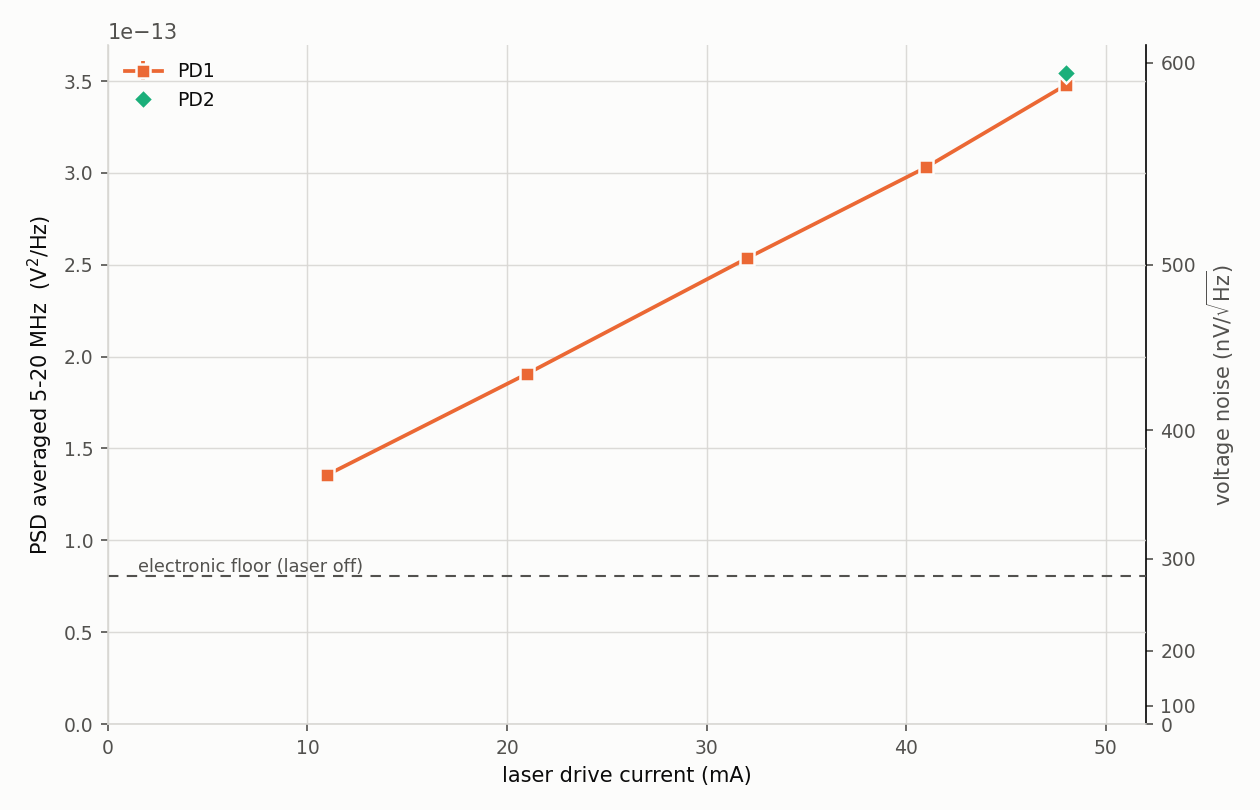
\includegraphics[width=1\linewidth]{psd_vs_current_single.png}
	\caption{A3: 5 - 20MHz Average PSD vs Laser Current with Single-Ended Detection}
	\label{fig:A3Plot}
\end{figure}

It can be seen in \autoref{fig:A3Plot} that indeed, the total noise is lower than in \autoref{fig:A2PSDvsCurrent}, as expected. Observing the total noise at the operating point of 48mA however, it can be seen that a value of approximately $3.5 \times 10^{-13}V^2/Hz$ is obtained, which gives $2.694\times 10^{-13}V^2/Hz$ once electronic noise has been subtracted. In the balanced detection case at the same laser current, a value of $5.49\times10^{-13}V^2/Hz$ was obtained - subtracting electronic noise and halving this gives $2.342\times 10^{-13}V^2/Hz$. This clearly indicates that the noise power in the single-ended case is higher than simply half of the shot-noise in the balanced detection case, thus proving that indeed there is excess RIN present. This excess RIN noise can be calculated:
\begin{equation}
	RIN_{excess}= (2.694 - 2.342)\times 10^{-13} = 0.352\times 10 ^{-13}V^2/Hz
\end{equation}

Converting to dB:

\begin{equation}
	10log_{10}(1+\frac{RIN_{excess}}{S})=10log_{10}(1+\frac{0.352\times 10 ^{-13}}{2.324\times 10^{-13}})= 0.6125dB
\end{equation}

Thus, RIN contributes an additional 0.6125dB of noise above the ideal shot-noise limit at the 48mA operating point. Balanced detection allows this excess noise to be removed, as illustrated in the results of A2 - allowing for a better SNR.
